% The determinism square: replaying the trace and resuming from a checkpoint reach
% the SAME working set at cursor c (commutes), because residency is a function of the
% logical clock — not wall-time.
\documentclass[border=8pt]{standalone}
\usepackage{tikz}
\usetikzlibrary{arrows.meta, positioning}
\usepackage{xcolor}
\definecolor{cc}{HTML}{4F46E5}
\definecolor{gg}{HTML}{16A34A}
\begin{document}
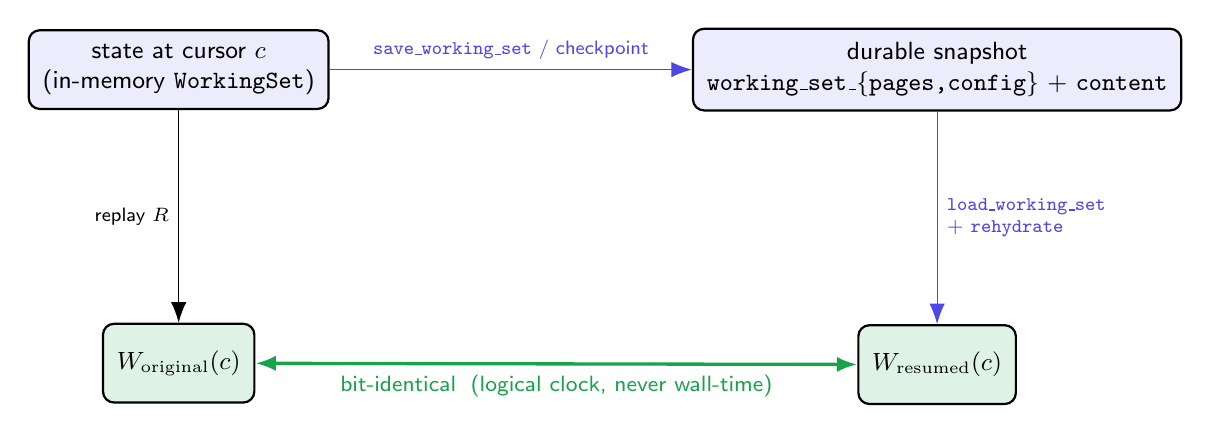
\begin{tikzpicture}[font=\sffamily\small, node distance=2.7cm and 4.6cm,
    box/.style={draw, thick, rounded corners, fill=#1, minimum height=10mm, align=center, inner sep=5pt},
    >={Latex[length=2.6mm]}]
  \node[box=cc!10] (tl) {state at cursor $c$\\(in-memory \texttt{WorkingSet})};
  \node[box=cc!10, right=of tl] (tr) {durable snapshot\\\texttt{working\_set\_\{pages,config\}} $+$ \texttt{content}};
  \node[box=gg!14, below=of tl] (bl) {$W_{\mathrm{original}}(c)$};
  \node[box=gg!14, below=of tr] (br) {$W_{\mathrm{resumed}}(c)$};

  \draw[->, cc] (tl) -- node[above, font=\sffamily\scriptsize]{\texttt{save\_working\_set} / checkpoint} (tr);
  \draw[->] (tl) -- node[left, font=\sffamily\scriptsize]{replay $R$} (bl);
  \draw[->, cc] (tr) -- node[right, font=\sffamily\scriptsize, align=left]{\texttt{load\_working\_set}\\$+$ \texttt{rehydrate}} (br);
  \draw[<->, gg, very thick] (bl) -- node[below, gg, font=\sffamily\footnotesize]{bit-identical \;(logical clock, never wall-time)} (br);
\end{tikzpicture}
\end{document}
